\subsection{Impact of CUPA Heuristics and Interpreter Optimizations}
\label{sec:sub:perf-cupa}

We now analyze the impact of the CUPA heuristics (described in Section~\ref{sec:chef:cupa}) and the interpreter optimizations (described in Section~\ref{sec:chef:optimizeforsymbex}) on test generation effectiveness.  Specifically, we measure the number of paths (respectively source code lines) covered by the test suite generated in 30 minutes for the packages in Table~\ref{tab:targets}.

We compare the results obtained in 4 different configurations: (1) the baseline, consisting of performing random state selection while executing the unmodified interpreter, and then either use (2) the path- or coverage-optimized CUPA only, (3) the optimized interpreter only, or (4) both CUPA and the optimized interpreter.  This way we measure the individual contribution of each technique, as well as their aggregate behavior.

\paragraph{Test Case Generation}

Figure~\ref{fig:tc-improv} compares the number of test cases generated with each of the 4 \chef configurations, using the path-optimized CUPA~(Section~\ref{sec:chef:cupa-paths}).  We only count the \textit{relevant} high-level test cases, that is, each test case exercises a unique high-level path in the target Python program.

\begin{figure}
  \centering
  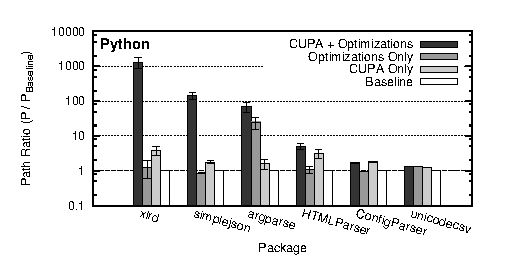
\includegraphics[width=0.7\textwidth]{evaluation/graphs/chef/bkdown-path-python} \\
  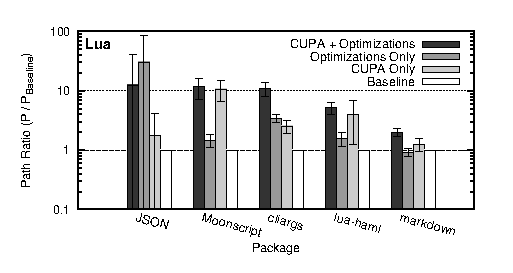
\includegraphics[width=0.7\textwidth]{evaluation/graphs/chef/bkdown-path-lua}
  \caption{The number of Python and Lua test cases generated by coverage- and path-optimized CUPA relative to random state selection (logarithmic scale).}
  \label{fig:tc-improv}
\end{figure}

For all but one of the 11 packages (6 Python plus 5 Lua), the aggregate CUPA + interpreter optimizations performs the best, often by a significant margin over the baseline.  This validates the design premises behind our techniques.

The CUPA strategy and the interpreter optimizations may interact non-linearly.  In two cases (Python's \codebit{xlrd} and \codebit{simplejson}), the aggregate significantly outperforms either individual technique. These are cases where the result is better than the sum of its parts.  In the other cases, the result is roughly the sum of each part, although the contribution of each part differs among targets.  This is visually depicted on the log-scale graph: for each cluster, the heights of the middle bars measured from level $1 \times$ roughly add up to the height of the aggregate (left) bar.

In one case (Lua's \codebit{JSON}), the aggregate performs worse on average than using the interpreter optimizations alone.  Moreover, the performance of each configuration is less predictable, as shown by the large error bars.  This behavior is due to the generated tests that cause the interpreter to hang, as explained in Section~\ref{sec:eval:bug-finding}.  To detect hangs, the test runs for 60 seconds before switching to another test case.  This acts as a ``penalty'' for the configurations that find more paths leading to the hang and also skews the distribution of path execution times, since the hanging paths take significantly longer than the normal (terminating) paths.

\paragraph{Line Coverage}

Figure~\ref{fig:coverage-improv} shows the line coverage achieved by each configuration, using CUPA optimized for line coverage (Section~\ref{sec:chef:cupa-coverage}).  In 6 out of 11 packages, the coverage improvement is noticeable, and for Python's \codebit{simplejson} and \codebit{xlrd}, the improvements are significant ($80\%$ and $40\%$).

Note that these coverage improvements are obtained using basic symbolic tests that do not make assumptions about the input format.  We believe that tailoring the symbolic tests to the specifics of each package could improve these results significantly.

\begin{figure}
  \centering
  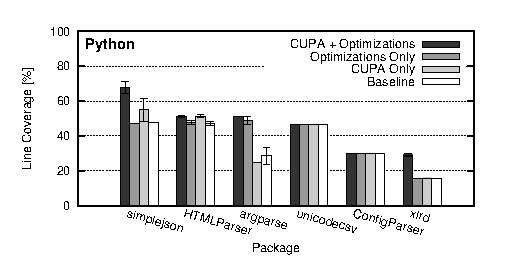
\includegraphics[width=0.7\textwidth]{evaluation/graphs/chef/bkdown-stmtcov-python} \\
  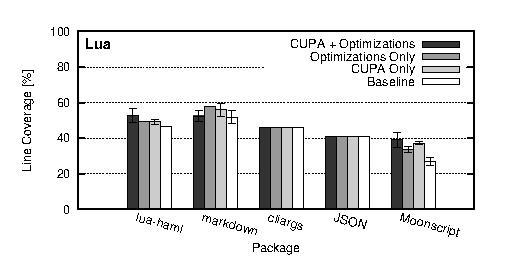
\includegraphics[width=0.7\textwidth]{evaluation/graphs/chef/bkdown-stmtcov-lua}
  \caption{Line coverage for the experiments of Figure~\ref{fig:tc-improv}.}
  \label{fig:coverage-improv}
\end{figure}

\subsection{Breaking Down Chef's Interpreter Optimizations}
\label{sec:sub:optimizations}

We now analyze in more depth the impact of the interpreter optimizations by breaking them down into the three types mentioned in Section~\ref{sec:chef:optimizeforsymbex}: avoiding symbolic pointers, hash neutralization, and fast-path elimination.  We run again the symbolic tests for 30 minutes, using the path-optimized CUPA and four different interpreter builds, starting from the vanilla interpreter and adding the optimization types one by one.  For each build and package, we count the number of high-level paths discovered by \chef.

Figure~\ref{fig:optimizations} shows the results for Python.  The data is normalized such that the number of high-level paths for each target reaches $100\%$.  For 3 out of 6 packages (\codebit{simplejson}, \codebit{argparse}, and \codebit{HTMLParser}), \chef's performance monotonically increases as more optimizations are introduced.  For \codebit{unicodecsv} and \codebit{ConfigParser}, the optimizations do not bring any benefits or even hurt slightly.  

However, in the case of \codebit{xlrd}, hash neutralization and fast path elimination seem to actually \emph{hurt} symbolic execution, since the best performance is attained when only symbolic pointer avoidance is in effect.  We explain this behavior by the fact that the different optimization levels cause the search strategy to explore different behaviors of the target package.  \codebit{xlrd} is by far the largest Python package in our evaluation (7.2KLOC vs. the second largest of 1.4KLOC) and includes a diverse set of behaviors, each with its own performance properties.

This result suggests that, for large packages, a \emph{portfolio} of interpreter builds with different optimizations enabled would help further increase the path coverage.

\begin{figure}
  \centering
  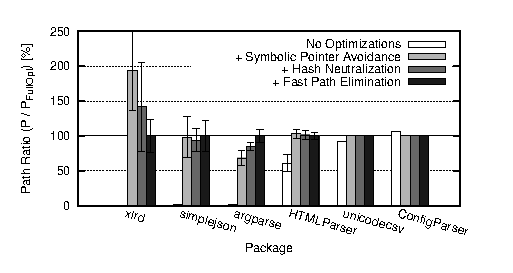
\includegraphics[width=0.7\textwidth]{evaluation/graphs/chef/optimizations-bars-python}
  \caption{The contribution of interpreter optimizations for Python as number of high-level paths explored.  Number of paths is relative to full optimizations ($100\%$) for each package.}
  \label{fig:optimizations}
\end{figure}


\subsection{Comparing Chef Against Hand-Made Engines}
\label{sec:sub:comparison}

We now evaluate the trade-offs in using a symbolic execution engine generated with \chef over building one ``by hand''.

\paragraph{Hand-Made Engines}

To our knowledge, no symbolic execution engine for Lua exists.  For Python, we found three research tools, which we compare \chef to.  (1) \cutiepy~\cite{cutie-py} is a concolic engine based on a formal model of the Python language.  It uses a custom CPython interpreter to drive a concrete execution, along with updating the symbolic state according to model semantics. (2) NICE-PySE~\cite{nice} is part of the NICE framework for testing OpenFlow applications.  We will refer to it as \nicese, for brevity. It wraps supported data types into symbolic counterparts that carry the symbolic store, and uses Python's tracing mechanisms to implement the interpretation loop fully in Python.  (3) The symbolic execution engine of the scalability testing tool Commuter~\cite{commuter} is also entirely built in Python.  Its primary purpose is the construction of models that explicitly use an API of symbolic data types.

We perform our comparison along three aspects: language features supported, implementation faithfulness, and performance.  The last two aspects are evaluated only against \nicese, which, besides being open source, is most compatible with our symbolic data representation (based on STP~\cite{stp}).

\paragraph{Language Feature Support}

Table~\ref{tab:langfeats} summarizes the language feature support for \chef, \nicese, \cutiepy, and \commuterse, as implemented at the moment of writing.  We relied on information from the respective papers in all cases and additionally on the implementation in the cases of \nicese and \commuterse, which are available as open source.

We distinguish engines designed to support arbitrary Python code (the ``Vanilla'' label) and those where the symbolic data types are an API used by model code (the ``Model'' label).  Engines in the ``Model'' category essentially offer a ``symbolic domain-specific language'' on top of the interpreted language.  \chef, \cutiepy, and \nicese are ``vanilla'' engines, since their testing targets do not have to be aware that they are being symbolically executed.  \commuterse is a model-based engine, since its testing targets are bound to the symbolic API offered by the engine.

We grouped the supported language features into program state representation (the language data model and types) and manipulation (the operations on data).  We divide data types into values (integers, strings and floating-point), collections (lists and dictionaries), and user-defined classes.  The operations consist of data manipulation, basic control flow (e.g., branches, method calls), advanced control flow (e.g., exception handling, generators), and native method invocations (they are atomic operations at the high level).  We also include in the comparison the ability to execute unsupported operations in concrete-only mode.


% Some names unlikely to clash with other definitions...
\newcommand{\compsupp}{\ensuremath{\CIRCLE}}
\newcommand{\partsupp}{\ensuremath{\LEFTcircle}}
\newcommand{\unsupp}{\ensuremath{\Circle}}

\begin{table}[tb]
\centering
\small
\begin{tabular}{@{\hspace*{2pt}}l@{\hspace*{2pt}} | @{\hspace*{2pt}}c@{\hspace*{2pt}} | @{\hspace*{2pt}}c@{\hspace*{2pt}} | @{\hspace*{2pt}}c@{\hspace*{2pt}} | @{\hspace*{2pt}}c@{\hspace*{2pt}}}
                    & \textbf{\chef}            & \textbf{\cutiepy} & \textbf{\nicese} & \textbf{\commuterse} \\
\hline
\rule{0pt}{12pt}\textbf{Engine type}& Vanilla   & Vanilla    & Vanilla   & Model       \\
\rule{0pt}{12pt}\textbf{Data types} &           &            &           &             \\
Integers            & $\compsupp^{\hphantom{*}}$  & \compsupp  & \compsupp  & \compsupp  \\
Strings             & $\compsupp^{\hphantom{*}}$  & \unsupp    & \unsupp    & \partsupp  \\
Floating point      & $\unsupp^{\hphantom{*}}$    & \unsupp    & \unsupp    & \unsupp    \\
Lists and maps      & $\compsupp^{*}$           & \partsupp   & \unsupp    & \compsupp  \\
User-defined classes& $\compsupp^{*}$           & \unsupp     & \partsupp   & \partsupp \\
\rule{0pt}{12pt}\textbf{Operations}   &                          &            &            &             \\
Data manipulation     & $\compsupp^{\hphantom{*}}$ & \partsupp  &  \partsupp & \partsupp   \\
Basic control flow    & $\compsupp^{\hphantom{*}}$ & \compsupp  &  \partsupp & \compsupp   \\
Advanced control flow & $\compsupp^{\hphantom{*}}$ & \compsupp  &  \unsupp   & \compsupp   \\
Native methods        & $\compsupp^{\hphantom{*}}$ & \partsupp  &  \unsupp   & \unsupp     \\
\end{tabular}
\rule{0pt}{12pt}\compsupp Complete \hspace{12pt} \partsupp Partial \hspace{12pt} \unsupp Not supported
\caption{Language feature support comparison for \chef and dedicated Python symbolic execution engines.  %% A full bullet means complete concrete and symbolic support for the feature available in the implementation.  A half-full bullet means a partial implementation, while an empty bullet means no support for the feature.
  Complete support with (*) refers to the internal program data flow and not to the initial symbolic variables.}
\label{tab:langfeats}
\end{table}

In a nutshell, \cutiepy is able to complete correctly any execution in concrete mode by using the interpreter implementation directly.   However, the symbolic semantics for each data type and native function must be explicitly provided by the developer, which makes \cutiepy impractical to use with rich Python applications.  \nicese suffers from the additional limitation that it has to support each bytecode instruction explicitly, which makes the tool impossible to use beyond its target applications.  Finally, \commuterse provides a rich set of symbolic data types, including lists and maps, by taking advantage of Z3's extended support for arrays~\cite{general-arrays}.  However, it supports only Python programs explicitly written against its API and does not handle native functions.

%% \cutiepy supports the semantics of integers, maps, and lists.  Other data types are supported as uninterpreted types, whose objects are opaque except for their identity.  Other data structures may be added to the model, expressed as uninterpreted functions and arrays.  By using the interpreter implementation to drive the concrete execution, \cutiepy is able to complete correctly any execution in concrete mode, while the symbolic evaluation and branching is limited to what the model offers.

%% \nicese supports only integers and Ethernet frame headers (encapsulated in a class) as symbolic data types, since they are required by the targeted OpenFlow switch applications.  Similarly, the supported operations include those encountered in the target applications.  This leaves out the support for advanced control flow and native methods (other than the built-in calls required by the supported data types).  By using its own (incomplete) interpretation loop, \nicese is not able to fall back on concretizing unsupported operations and so terminates the execution with an error in such cases.

%% \commuterse takes advantage of Z3's extended support for arrays~\cite{general-arrays} to efficiently model lists and maps, in addition to integers.  The support for strings is partially provided by uninterpreted types, which can only reason about object equality.  Moreover, the uninterpreted types can be used as keys in symbolic maps, which allows data structures such as file directories used in the POSIX model.

The engine generated by \chef offers complete symbolic support for almost all language features.  Floating point operations are supported only concretely, due to lack of support in STP, the constraint solver used by S2E.  For the same reasons, the symbolic program inputs can only be integers and strings.  However, all data structures are supported during the execution.

Each half or empty bullet in Table~\ref{tab:langfeats} implies that significant engineering effort would be required to complete a feature.  While useful for their evaluation targets, \nicese and \cutiepy are unable to handle a complex software package that makes use of Python's many language features.


\paragraph{Use as Reference Implementation}

When the need for performance justifies investing in a dedicated engine implementation, an engine created from \chef can serve as a reference implementation during development.  One can find bugs in a symbolic execution engine by comparing its test cases with those generated by \chef.  The process can be automated by tracking the test cases generated by the target engine along the high level paths generated by \chef to determine duplicates and missed feasible paths.

%% To automate the engine comparison, we augmented \chef with test case ``seeding''. The tests generated with the target engine (\nicese) are fed to \chef as ``seeds'',  which are tracked along the high-level paths generated by \chef.  A seed test follows a high-level path if the test input matches the path constraint.  If the target engine is correct, each \chef high-level path should track exactly one seed.  More seeds per path indicate test case duplication, while zero seeds flags a missed path.

In this mode, we found a bug in the \nicese implementation, which was causing it to generate redundant test cases and miss feasible paths.  The bug was in the way \nicese handled \codebit{if not <expr>} statements in Python, causing the engine to select for exploration the wrong branch alternate and end up along an old path.  We are assisting the \nicese developers in identifying and fixing any other such bugs.

In conclusion, the experiment provides evidence that a system combining an established low-level symbolic execution engine (e.g., S2E) with a reference interpreter implementation is more robust than a symbolic execution engine built from scratch.


%% \johannes{This entire section is strange, because we evaluate this only for NICE, whereas we claimed initially that we would evaluate correctness against all engines}


\paragraph{Performance}

The downside of \chef is that the symbolic execution engines produced are slower than their hand-written equivalents.  We quantify this drawback by applying \chef to the experimental setup of \nicese, consisting of an OpenFlow switch controller program that implements a MAC learning algorithm.  The controller receives as input a sequence of Ethernet frames and, in response, updates its forwarding table (stored as a Python dictionary).  We use symbolic tests that supply sequences of between 1 and 10 Ethernet frames, each having the MAC address and frame types marked as symbolic.

\begin{figure}
  \centering
  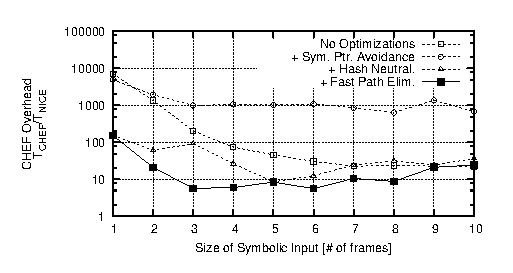
\includegraphics[0.7\textwidth]{evaluation/graphs/chef/nice-optimizations}
  \caption{Average overhead of \chef compared to \nicese, computed as ratio of average per-path execution times.  The average divides total tool execution time by number of high-level paths generated.}
  \label{fig:nice-overhead}
\end{figure}

Given the small size of the controller (less than 100~LOC), the number of execution paths is relatively small, and choosing low-level paths at random quickly discovers new high-level paths.  Therefore, the search strategy has no impact (in the experiments we used path-optimized CUPA).  However, the interpreter optimizations are crucial, since the controller code relies heavily on the dictionary.  As in Section~\ref{sec:sub:optimizations}, we use several interpreter builds with optimizations introduced one-by-one.

Figure~\ref{fig:nice-overhead} illustrates the overhead for each optimization configuration, as a function of number of Ethernet frames supplied.  The overhead is computed as the ratio between the average execution times per high-level path of \nicese and \chef.  In turn, the execution time per high-level path is computed by dividing the entire execution time of each tool by the number of paths it produced.

%% Basically the same reasons we already gave earlier in the paper

The performance of each optimization configuration illustrates the sources of path explosion and slowdown in the vanilla interpreter.  With no optimizations, symbolic keys in the MAC dictionary cause massive path explosion due to symbolic pointers.  When avoiding symbolic pointers, performance drops even more due to symbolic hash computations.  This penalty is reduced up to two orders of magnitude with hash neutralization.  Finally, fast path elimination reduces the forking inside string key comparisons in the dictionary.

The shape of the final performance curve (the solid line) is convex.  For 1 and 2 symbolic frames, the search space is quickly exhausted and the execution time is dominated by \chef's initialization costs, i.e., setting up the symbolic VM and executing the interpreter initialization inside the guest.  This results in an execution overhead as high as $120 \times$.  For more symbolic frames, the initialization cost is amortized, and the overhead goes below $5 \times$.  However, as the number of frames increases, so does the length of the execution paths and the size of the path constraints, which deepens the gap between \chef's low-level reasoning and \nicese's higher level abstractions.  For 10 symbolic frames, the overhead is around $40 \times$.

Despite \chef's performance penalty, the alternative of writing an engine by hand is daunting. It involves developing explicit models that, for a language like Python, are expensive, error-prone, and require continuous adjustments as the language evolves.
%
Where performance is crucial, a hand-written engine is superior; however, we believe that \chef is a good match in many cases.

%%% Local Variables: 
%%% mode: latex
%%% eval: (visual-line-mode)
%%% fill-column: 1000000
%%% TeX-master: "main"
%%% End:
